\subsection{ASTEKA Project}
A member of the MMEA project, the research group of Environmental Informatics at the University of Eastern Finland (Kuopio campus) has a project called ASTEKA. The project aims at commercializing a monitoring system of living health and energy efficiency. \cite{Asteka10} Basically, the project equips houses with sensors that provide informative online data presentations for the resident of the house. By monitoring different variables, such as energy consumption and $CO_2$ levels, the house or the resident could adjust the control variables accordingly. 

Their first pilot was introduced at a living fare in Kuopio in the summer of 2010. The pilot originally consisted of 11 houses each of which has sensors ranging from $CO_2$ concentration and temperature to electricity and water consumption. The web interface of the pilot shows daily, weekly and monthly consumption statistics and charts which can be used to improve energy efficiency. \cite{Asteka10} For example, one can easily notice whether the sudden peak in electricity consumption is caused by falling outside temperature or excessive oven usage.


\subsection{Test House and Sensors}
In this thesis I use data from one of the pilot houses. The house has three floors and sensors in all of them. The layout of the first floor is presented in Figure~\ref{fig:floor1}. The squares with numbers in them are sensor units which are listed in Table~\ref{table:floor1}.

\begin{figure}[here]
\centering
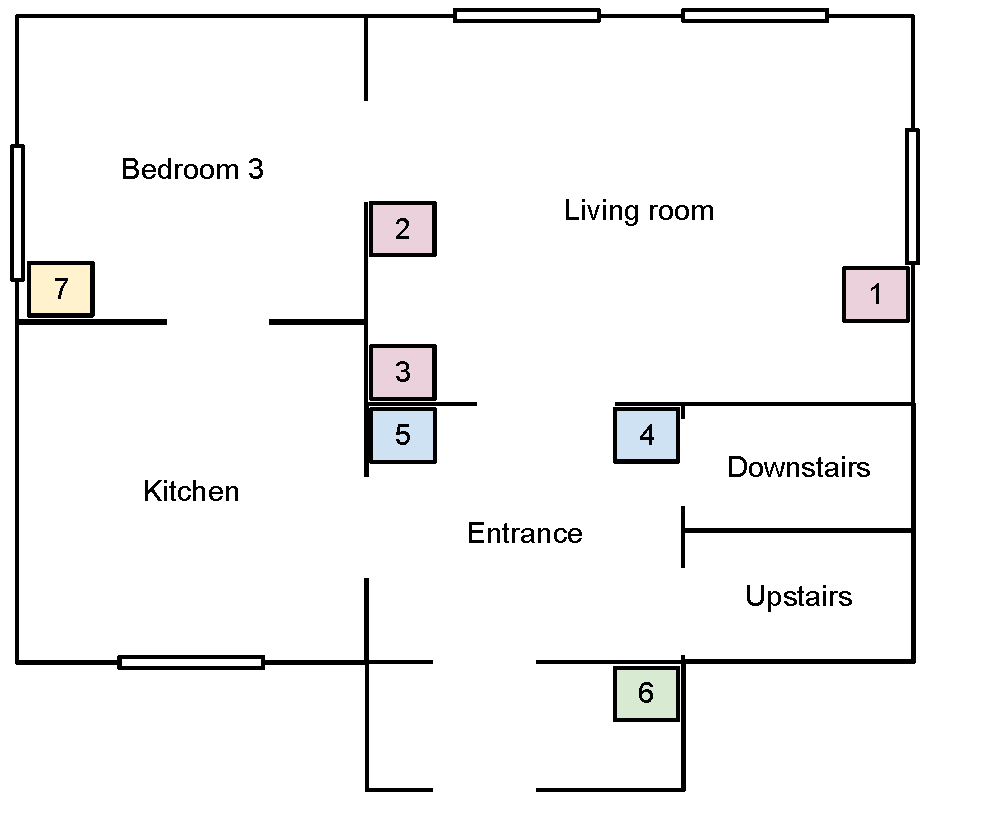
\includegraphics[scale=0.7]{images/keskikerros.pdf}
\caption{Layout of the first floor and the locations of the sensor units.}
\label{fig:floor1}
\end{figure}

The second floor, which has only 2 sensor units, is shown in Figure~\ref{fig:floor2} and its sensors are listed in Table~\ref{table:floor2}. Both the two sensors in the second floor are located in bedrooms. However, bedroom 3 serves as a guest room and thus is empty most of the time, which should be detected in the data easily.

\begin{figure}[here]
\centering
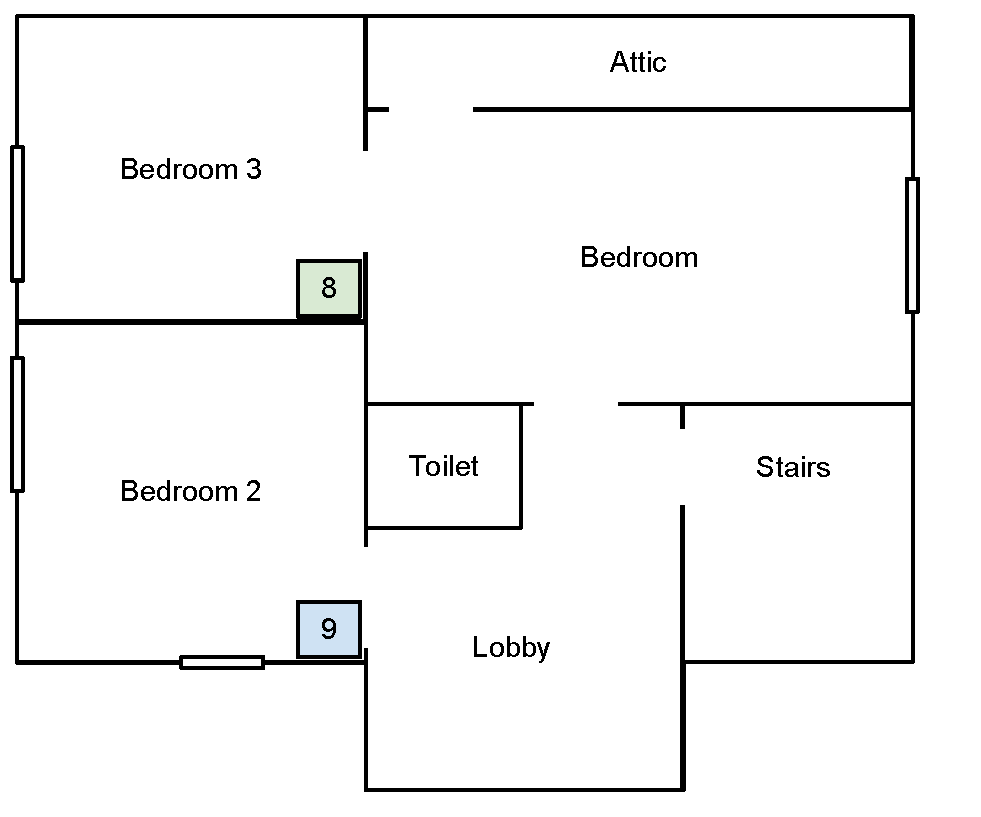
\includegraphics[scale=0.7]{images/ylakerta.pdf}
\caption{Layout of the second floor and the locations of the sensor units.}
\label{fig:floor2}
\end{figure}

In the basement most of the sensors are located in the boiler room which is a well isolated space with no windows. The layout of the basement is presented in Figure~\ref{fig:basement}. The listing of the sensors in the basement is shown in Table~\ref{table:basement}. An interesting detail in the basement is how the sensor unit 10 with humidity and temperature sensors is placed near the showers and the sauna. This should definitely be shown somehow in the data from these sensors.

\begin{figure}[here]
\centering
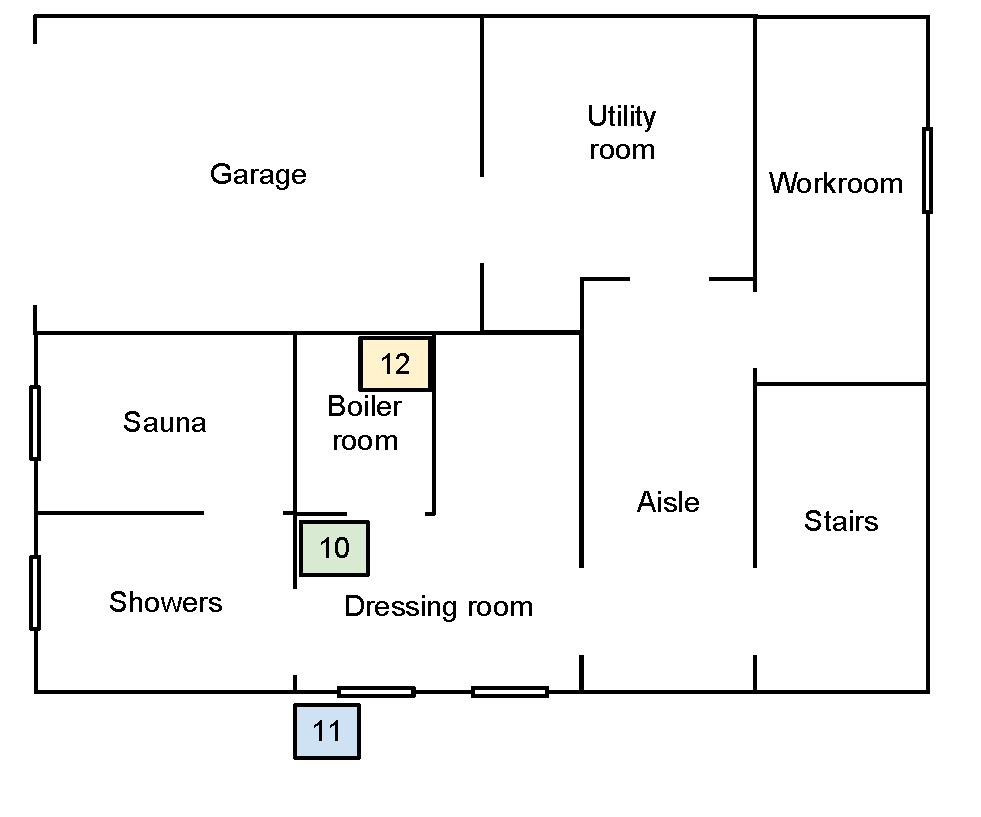
\includegraphics[scale=0.7]{images/kellari.pdf}
\caption{Layout of the basement and the locations of the sensor units.}
\label{fig:basement}
\end{figure}



\begin{table}
  \caption{Sensors in the first floor of the test house} 
  \begin{tabular}{l | l | l | l | c}
    \multicolumn{4}{l}{\textbf{First floor}} \\
    \hline
   	\textbf{Room} & \textbf{Group} & \textbf{Sensor ID} & \textbf{Variable} & \textbf{Unit} \\
    \hline
    Living room & 1 & 51 & Temperature & $^\circ C$ \\
    \hline
    Living room & 2 & 52 & $CO$ & ppm \\
    \hline
    Living room & 3 & 815 & PIR & ON/OFF \\
      &  & 815 & Humidity & \%RH \\
      &  & 817 & Temperature & $^\circ C$ \\
      &  & 818 & $CO_2$ OH & ppm \\
    \hline
    Inner entrance & 4 & 53 & Temperature ET & $^\circ C$ \\
      &  & 54 & Humidity ET & \%RH \\
      &  & 55 & $CO_2$ & ppm \\
      &  & 60 & Electricity & Wh \\
    \hline
    Inner entrance & 5 & 844 & Small particles & count / $ft^3$ \\
     & & 845 & Large particles & count / $ft^3$ \\
    \hline
    Outer entrance & 6 & 56 & Diff Pressure & Pa \\
    \hline
    Bedroom 3 & 7 & 650 & Temperature & $^\circ C$ \\
     & & 651 & Humidity & \%RH \\
     & & 652 & $CO_2$ & ppm \\
     & & 789 & VOC & ppm \\
  \end{tabular}
  \label{table:floor1}
\end{table}

\begin{table}
  \caption{Sensors in the second floor of the test house} 
  \begin{tabular}{l | l | l | l | c}
    \multicolumn{4}{l}{\textbf{Second floor}} \\
    \hline
   	\textbf{Room} & \textbf{Group} & \textbf{Sensor ID} & \textbf{Variable} & \textbf{Unit} \\
    \hline
    Bedroom 1 & 8 & 644 & Humidity & \%RH \\
     & & 645 & Temperature & $^\circ C$ \\
     & & 646 & $CO_2$ & ppm \\
    \hline
    Bedroom 2 & 9 & 647 & Humidity & \%RH \\
     & & 648 & Temperature & $^\circ C$ \\
     & & 649 & $CO_2$ & ppm \\
    \hline
  \end{tabular}
  \label{table:floor2}
\end{table}


\begin{table}
  \caption{Sensors in the basement of the test house} 
  \begin{tabular}{l | l | l | l | c}
    \multicolumn{4}{l}{\textbf{Basement}} \\
    \hline
   	\textbf{Room} & \textbf{Group} & \textbf{Sensor ID} & \textbf{Variable} & \textbf{Unit} \\
    \hline
    Dressing room & 10 & 57 & Humidity & \%RH \\
     & & 58 & Temperature & $^\circ C$ \\
     & & 59 & $CO_2$ & ppm \\
    \hline
    Outside & 11 & 772 & Temperature & $^\circ C$ \\
    \hline
    Boiler room & 12 & 62 & Water & $m^3$ \\
    & & 773 & Floor heating outgoing water & $^\circ C$ \\
    & & 775 & Floor heating & $^\circ C$ \\
    & & 776 & L1 indoor temperature, incoming & $^\circ C$ \\
    & & 777 & Used water & $^\circ C$ \\
    & & 778 & Variable & $^\circ C$ \\
    & & 779 & Radiator outgoing water & $^\circ C$ \\
    & & 783 & Hot water & \% \\
    & & 784 & Radiator indoor temperature & $^\circ C$ \\
    & & 785 & District heating incoming temperature & $^\circ C$ \\
    & & 786 & District heating return temperature & $^\circ C$ \\
    & & 787 & District heating energy & kWh \\
    & & 788 & District heating water flux & $m^3$ \\
  \end{tabular}
  \label{table:basement}
\end{table}

\subsection{Test Data}
The data from ASTEKA server is available via a Java library. The library allows one to specify two dates and it downloads two types of files, sensor files and measurement files. The sensor files are of the following form:

\begin{description}
\item[Filename:]{sensors8\_11.txt}
\item[Header:]{SensorID:int; name:varchar(100)}
\item[Example line:]{51;Temperature Fileplace (Har 1)}
\end{description}

The file name contains to identification numbers: the former is a house ID and the latter is sensor group ID. The header line specifies the columns used in the file but since they are similar in each sensor file, they do not need to be read. The example line shows that the columns are separated by a semicolon.

The measurement files are of the following form:

\begin{description}
\item[Filename:]{measurements8\_11.txt}
\item[Header:]{unixtime(BIGINT); ID\_8\_11\_51(DOUBLE), ID\_8\_11\_52(DOUBLE); ...}
\item[Example line:]{1356998401;21.0253;0.0032; ...}
\end{description}


Like the sensor file names, the measurement file names contain a house ID and a sensor group ID. Again, the header line specifies the columns found in the file. The first column is always an Unix timestamp which tells how many seconds have passed since 1.1.1970 until the the measurement was made. The rest of the columns specify the IDs and the types of the values the sensor is emitting. The numbers in pattern \emph{ID\_8\_11\_51} are house ID, sensor group ID and sensor ID, respectively. After that there is the variable type specified.

The complex events we are trying to detect are defined in Chapter 4.4.

